\documentclass{article}

\usepackage[utf8]{inputenc}
\usepackage[ngerman]{babel}
\usepackage{amssymb}
\usepackage{amsmath}
\usepackage{graphics}
% Pseudocode
\usepackage{algorithm}
\usepackage[noend]{algpseudocode}
\usepackage{graphicx}
\usepackage{pdfpages}

\usepackage{tikz}

\setlength{\parindent}{0in}

\newcommand{\zettelNummer}{1}
\newcommand{\studierenderEins}{Eli Kogan-Wang (7251030)}
\newcommand{\studierenderZwei}{David Noah Stamm (7249709)}
\newcommand{\studierenderDrei}{Bogdan Rerich (7248483)}
\newcommand{\studierenderVier}{Jan Schreiber()}

\newcounter{AufgabenCounter}
\setcounter{AufgabenCounter}{1}
\newcounter{TeilaufgabenCounter}
\newenvironment{aufgabe}{\section*{Aufgabe \theAufgabenCounter}\setcounter{TeilaufgabenCounter}{1}}{\stepcounter{AufgabenCounter}}
\newenvironment{teilaufgabe}{\paragraph*{\alph{TeilaufgabenCounter})}}{\stepcounter{TeilaufgabenCounter}}

\renewcommand{\to}{\textnormal{ to }}
\newcommand{\bigO}{\mathcal{O}}

\newcommand{\qed}{\hfill$\square$}

\begin{document}

\title{Berechnbarkeit und Komplexität \\ Heimübung \zettelNummer{}}
\author{\studierenderEins{} \\
  \studierenderZwei{} \\
  \studierenderDrei{} \\
  \studierenderVier{}}

\maketitle

% Aufgabe 1
\begin{aufgabe}

  Der Algorithmus \textsc{Bipartite-Check-Breadth-First-Search} nimmt einen Graphen $G$ und einen Startknoten $s\in V$.

  \begin{algorithm}[H]
    \caption{\textsc{Bipartite-Check-Breadth-First-Search}($G, s$)}
    \begin{algorithmic}[1]
      \For{jeden Knoten $u$ in $V\backslash\{s\}$}
      \State $color[u]\gets WHITE$
      \State $\pi[u]\gets NIL$
      \EndFor
      \State $color[s]\gets GRAY$
      \State $\pi[s]\gets NIL$
      \State $Q\gets\{\}$
      \State Enqueue($Q$, $s$)
      \While{$Q\neq\emptyset$}
      \State $u\gets$ Dequeue($Q$)
      \If{$color[u]=GRAY$}
      \State otherColor $\gets BLACK$
      \Else
      \State otherColor $\gets GRAY$
      \EndIf
      \For{jeden Knoten $v$ in $A(u)$} \Comment{$A(u)$: Nachbarn von $u$}
      \If{$color[v]=WHITE$}
      \State $color[v]\gets $ otherColor
      \State $\pi[v]\gets u$
      \State Enqueue($Q$, $v$)
      \ElsIf{$color[v]\neq$ otherColor}
      \State \textbf{return} \textsc{false}
      \EndIf
      \EndFor
      \EndWhile
      \State \textbf{Return} \textsc{true}
    \end{algorithmic}
  \end{algorithm}

  Wir reduzieren das Problem der Bipartitheitsprüfung auf den der $2$-Färbbarkeit.

  Mithilfe der Breitensuche könenn wir die $2$-Färbung auf $G$ versuchen und bei einem Konflikt
  abbrechen.

  Ein Graph ist genau dann $2$-Färbbar, wenn er bipartit ist.

  Unser Algorithmus ist damit korrekt, weil true rückgibt, genau dann wenn der Graph $2$-Färbbar ist.
  Und weil er false rückgibt, wenn der Graph nicht $2$-Färbbar ist.

  Die Laufzeit einer Breitensuche ist aus DuA mit $O(|V|+|E|)$ bekannt.
  Da wir hierbei nur um Elementare Operationen erweitert, weswegen die Laufzeit für diesen Algorthimus erhalten bleibt.
\end{aufgabe}
%Aufgabe 2
\begin{aufgabe}
  \begin{equation*}
    \begin{aligned}
      010: &                                                    \\
           & q_0 \triangleright  0  1  0                        \\
           & \triangleright  q_0 0  1  0                        \\
           & \triangleright  \sqcup  q_1 1  0                   \\
           & \triangleright  \sqcup  1  q_1 0                   \\
           & \triangleright  \sqcup  1  0  q_1 \sqcup           \\
           & \triangleright  \sqcup  1  q_3 0  \sqcup           \\
           & \triangleright  \sqcup  q_5 1  \sqcup  \sqcup      \\
           & \triangleright  q_5 \sqcup  1  \sqcup  \sqcup      \\
           & \triangleright  \sqcup  q_0 1  \sqcup  \sqcup      \\
           & \triangleright  \sqcup  \sqcup  q_2 \sqcup  \sqcup \\
           & \triangleright  \sqcup  q_4 \sqcup  \sqcup  \sqcup \\
           & \triangleright  q_6 \sqcup  \sqcup  \sqcup  \sqcup \\
    \end{aligned}
  \end{equation*}
  $$q_6=q_{\text{accept}}$$
  \begin{equation*}
    \begin{aligned}
      1011: &                                                       \\
            & q_0 \triangleright  1  0  1  1                        \\
            & \triangleright  q_0 1  0  1  1                        \\
            & \triangleright  \sqcup  q_2 0  1  1                   \\
            & \triangleright  \sqcup  0  q_2 1  1                   \\
            & \triangleright  \sqcup  0  1  q_2 1                   \\
            & \triangleright  \sqcup  0  1  1  q_2 \sqcup           \\
            & \triangleright  \sqcup  0  1  q_4 1  \sqcup           \\
            & \triangleright  \sqcup  0  q_5 1  \sqcup  \sqcup      \\
            & \triangleright  \sqcup  q_5 0  1  \sqcup  \sqcup      \\
            & \triangleright  q_5 \sqcup  0  1  \sqcup  \sqcup      \\
            & \triangleright  \sqcup  q_0 0  1  \sqcup  \sqcup      \\
            & \triangleright  \sqcup  \sqcup  q_1 1  \sqcup  \sqcup \\
            & \triangleright  \sqcup  \sqcup  1  q_1 \sqcup  \sqcup \\
            & \triangleright  \sqcup  \sqcup  q_3 1  \sqcup  \sqcup \\
            & \triangleright  \sqcup  q_7 \sqcup  1  \sqcup  \sqcup \\
    \end{aligned}
  \end{equation*}
  $$q_7=q_{\text{reject}}$$
  \begin{equation*}
    \begin{aligned}
      0110: &                                                            \\
            & q_0 \triangleright  0  1  1  0                             \\
            & \triangleright  q_0 0  1  1  0                             \\
            & \triangleright  \sqcup  q_1 1  1  0                        \\
            & \triangleright  \sqcup  1  q_1 1  0                        \\
            & \triangleright  \sqcup  1  1  q_1 0                        \\
            & \triangleright  \sqcup  1  1  0  q_1 \sqcup                \\
            & \triangleright  \sqcup  1  1  q_3 0  \sqcup                \\
            & \triangleright  \sqcup  1  q_5 1  \sqcup  \sqcup           \\
            & \triangleright  \sqcup  q_5 1  1  \sqcup  \sqcup           \\
            & \triangleright  q_5 \sqcup  1  1  \sqcup  \sqcup           \\
            & \triangleright  \sqcup  q_0 1  1  \sqcup  \sqcup           \\
            & \triangleright  \sqcup  \sqcup  q_2 1  \sqcup  \sqcup      \\
            & \triangleright  \sqcup  \sqcup  1  q_2 \sqcup  \sqcup      \\
            & \triangleright  \sqcup  \sqcup  q_4 1  \sqcup  \sqcup      \\
            & \triangleright  \sqcup  q_5 \sqcup  \sqcup  \sqcup  \sqcup \\
            & \triangleright  \sqcup  \sqcup  q_0 \sqcup  \sqcup  \sqcup \\
            & \triangleright  \sqcup  \sqcup  \sqcup  q_6 \sqcup  \sqcup \\
    \end{aligned}
  \end{equation*}
  $$q_6=q_{\text{accept}}$$
\end{aufgabe}
%Aufgabe 3
\begin{aufgabe}
  informelle Beschreibung: \\ \\
  DTM bei Eingabe z $ \in {0,1,\#}$ \\
  Die DTM kann in 2 Phasen eingeteilt werden: \\ \\
  Phase 1 (pre prossessing): \\
  Teste, ob genau eine "\#" in der Eingabe vorkommt. Andernfalls verwerfe dieses. (Der Lesekopf wird wieder auf den Anfang des Wortes gesetzt). \\ \\
  Phase 2: \\
  Falls die Eingabe von der Form w\#x mit $w,x \in \{0,1\} $ ist, teste ob w=x gilt, indem jeweils Buchstabenweise w mit x verglichen wird. Ersetzte zu Vergleichende Buchstaben mit X. Falls nun Wort vollständig makiert ist, bis auf \#, so gilt w=x und die Eingabe ist in L \\ \\
  Formal: \\
  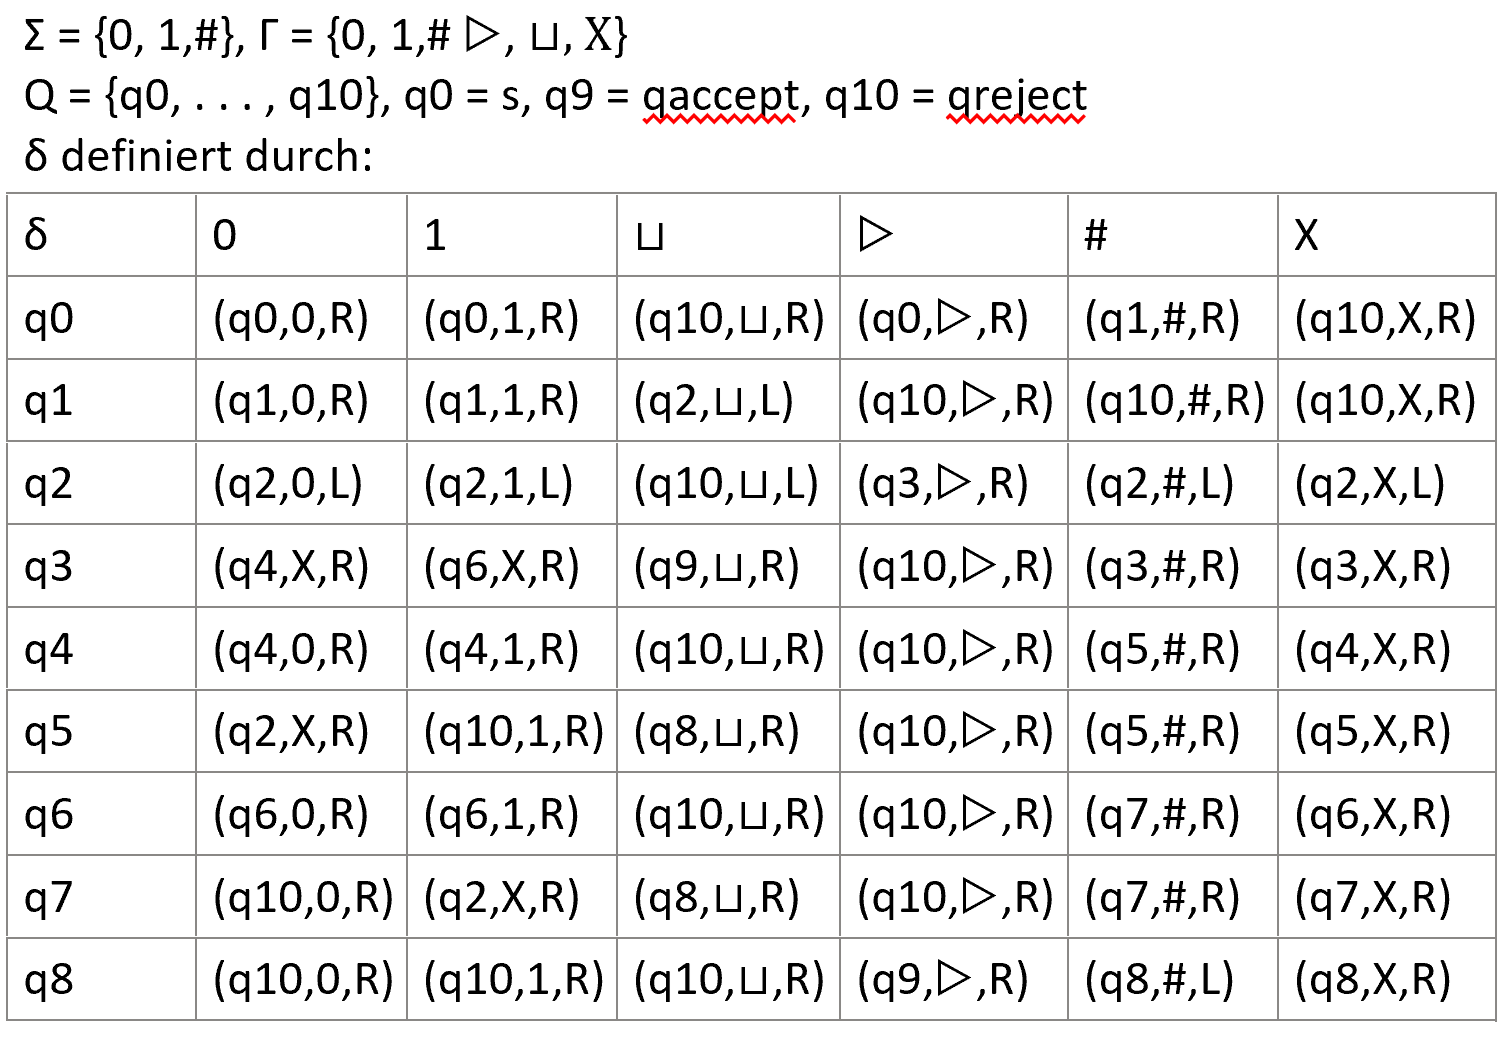
\includegraphics[scale=0.2]{image.png}
\end{aufgabe}
%Aufgabe 4
\begin{aufgabe}
  Annahme: $\delta$ ist zu jedem Zeitpunkt wohldefiniert. (d.h. das Beispielsweise ein Übergang, welcher links aus der Turingmaschine herausführen würde ist nicht in $\delta$ möglich.\\
  Zu zeigen: $$\forall \text{DTM}_\text{Abgewandelt}\,M\exists \text{DTM}_\text{Klassisch}\,M':\, L(M)=L(M')$$\\
  Gegeben sei $M=(\Sigma,\Gamma,Q,\delta)$ wie in der Aufgabe.

  Wir beschreiben den normalen DTM $M'=(\Sigma,\Gamma,Q',\delta')$. Mit:
  \begin{equation*}
    \begin{aligned}
      Q' & = (Q \backslash \{q_{\text{accept}},q_{\text{reject}}\}) \times \{L,\emptyset\} \cup \{q_{\text{accept}},q_{\text{reject}}\} \\
    \end{aligned}
  \end{equation*}
  \begin{equation*}
    \begin{aligned}
      \delta'((q,L),s)         & = ((q,\emptyset),s,L)                                                                     \\
      \delta'((q,\emptyset),s) & = \text{Sei } (q',s',d)=\delta(q,s) \text{ in }                                           \\
                               & \left\{\begin{aligned}
                                          (q_{\text{accept}},s',d) & \text{ falls } q' = q_{\text{accept}} \\
                                          (q_{\text{reject}},s',d) & \text{ falls } q' = q_{\text{reject}} \\
                                          ((q',L),s',L)            & \text{ falls } d = 2L                 \\
                                          ((q',\emptyset),s',R)    & \text{ falls } d = R                  \\
                                        \end{aligned}\right.
    \end{aligned}
  \end{equation*}

  Wobei der neue Startzustand $q_{\text{start}}'=(q_{\text{start}},\emptyset)$ ist.

  Unsere Turing Maschine ersetzt einen 2L Schritt durch einen L Schritt und einen im Zustand vermerkten L Schritt, der im nächsten Übergang ausgeführt wird.\\

  \textbf{Beweis:}

  Sei $w\in\Sigma*$.

  Nun seien $\begin{aligned}
      K_0=(q_{\text{start}}\triangleright w)   \\
      K_0'=(q_{\text{start}}'\triangleright w) \\
    \end{aligned}$ und $\begin{aligned}
      K_{i+1}\text{ Nachfolgekonfiguration von }K_i=(...q...)   \\
      K_{i+1}'\text{ Nachfolgekonfiguration von }K_i'(...q'...) \\
    \end{aligned}$ wenn $\begin{aligned}
      q_\text{accept}\neq q\neq q_\text{reject}  \\
      q_\text{accept}\neq q'\neq q_\text{reject} \\
    \end{aligned}$ und $\begin{aligned}
      K_{i+1}=K_i   \\
      K_{i+1}'=K_i' \\
    \end{aligned}$ sonst.

  Nun ist $g((\alpha(q',L)\beta))=0$, $g(K)=1$ sonst.
  Und $K''=(K_i'|g(K_i)=1\forall i)$.
  Nun ist $\Psi((\alpha q\beta))=\left\{\begin{aligned}
      (\alpha q\beta)             & \quad\text{wenn }q=q_\text{accept} \\
      (\alpha q\beta)             & \quad\text{wenn }q=q_\text{reject} \\
      (\alpha (q,\emptyset)\beta) & \quad\text{sonst}                  \\
    \end{aligned}\right.$

  Jetzt ist es vollkommen trivial, dass $\Psi(K_i)=K_i''$ für alle $i$.

  Damit ist $L(M)=L(M')$. \qed
  \\

  Wir haben im Beweis gezeigt, dass für alle Wörter, die Konfigurationsfolgen der Turingmaschinen, insofern man die hinzugefügten Zustände ignoriert, gleich sind.\\

  Insbesondere sind dann die Zustände $q_\text{accept}$ und $q_\text{reject}$ gleich auftretend bei $M$ und $M'$.\\
\end{aufgabe}
\end{document}